\documentclass[12pt]{article}

\usepackage{graphicx}
\usepackage{float}
\usepackage{amsmath}
\usepackage{amssymb}
\usepackage{graphicx}
\usepackage[utf8]{inputenc}
\usepackage[spanish]{babel}
\usepackage{geometry}
\geometry{left=2cm,right=2cm,top=2cm,bottom=2cm}
\usepackage{listings}
\lstset{basicstyle=\ttfamily,
  showstringspaces=false,
  commentstyle=\color{red},
  keywordstyle=\color{blue}
}


\title{%
  Proyecto 01\\
  \large Galería de arte \\
    \Large Computación Gráfica\\
     \large UNAM 2022-2}
\author{Gibran Zazueta Cruz \\
\small 09/junio/2022}
\date{}

\begin{document}
\maketitle

\section{Introducción}

Se utiliza OpenGL para crear una galeria virtual de arte compuesta de objetos 3D y shaders.

La exposición consiste de 8 objetos 3D. Los objetos se cargan de un formato wavefront obj y fueron en su mayoría obtenidos de internet. Se mecionan a continuación de acuerdo a sus posiciones

\begin{figure}[H]
\centering
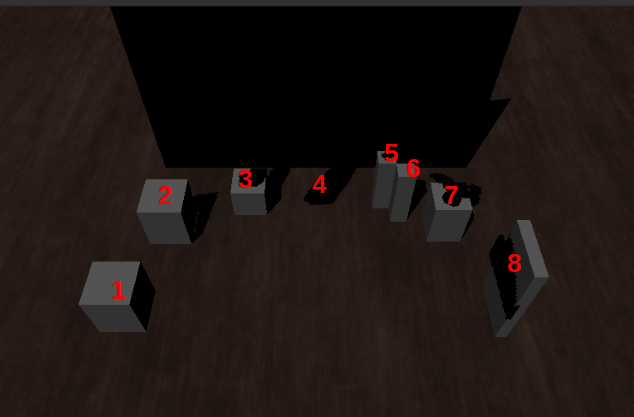
\includegraphics[scale=0.5]{images/posicion.png}
\caption{Posición de figuras en la escena}
\end{figure}

\begin{enumerate}

\item Conejo de stanford.
\item 'Vivi' (por 'Therealyton' en sketchfab)
\item Venus de milo (por la National Gallery of Denmark)
\item Estela maya (por Antoine Dresen)
\item 'Scholar'
\item Resting nude
\item Colorful rooster
\item Animación pizza
\end{enumerate}



\subsection{Texturizado}
Se utilizaron texturas para las paredes y el suelo. Estas fueron obtenidas de 3dtexture.com. 

Por otro lado, se mapea un 'skybox' con una textura cubemap alrededor de toda la escena 

El cubemap es un tipo de dato de extura que se compone de 6 texturas distintas, que representan los lados de un cubo. Una  ventaja de ellas es que sus cuyas coordenadas las define un vector de posición, que puede ser la posición dle fragmento. De esta manera, no es necesario especificar las coordenadas uv sobre la superficie. para realizar el mape de textura

\subsection{Shaders implementados}
Se implementaron los siguientes shaders:

\textbf{Phong (default) y phong con textura}
Se programó el modelo de iluminación de Phong con sus componenetes ambiental, difusa y especular. La implementación incluye la posibilidad de hacer sombreado con variane cantidad de luces y materiales.

\textbf{Mapa ambiental reflectivo}
Con ayuda de la textura cubemap se hace un mapeo ambiente sobre el objeto 1. Más específicamente el mapeo corresponde a un mapeo reflectivo. 

\textbf{Textura con animación}
Se crea una pequeña animación donde una textura es desplazada de acuero a una unidad de tiempo. La animación es actualizada cada frame

\textbf{Toon shader} 
Se realiza un toon shader básico forzando a la componente difusa a evitar la interpolación.

El modelo 1 utiliza el mapeo ambiental, el 8 la textura con animación y el 2 el toon shader. EL resto de los objetos utilizan el shader de phong con o sin textura.

\subsection{Luces}
Las luces utilizadas son una luz de sol (direccional para toda la escena) y luces seguidoras. Estas se implementaron con un ángulo de corte. Para las luces seguidoras se calculó una atenuación.

\subsection{Shadow Mapping}
Se implementa renderizado de sombras con la técnica de shadow mapping.- Al iniciar el programa se construye el mapa de profundidad en un framebuffer y se almacena en una textura de 2048x2048. Debido a que hay 15 luces se subdivide en mapara en 16 por lo que el mapa de sombras de cada luz es de 512x512.

\begin{figure}[H]
\centering
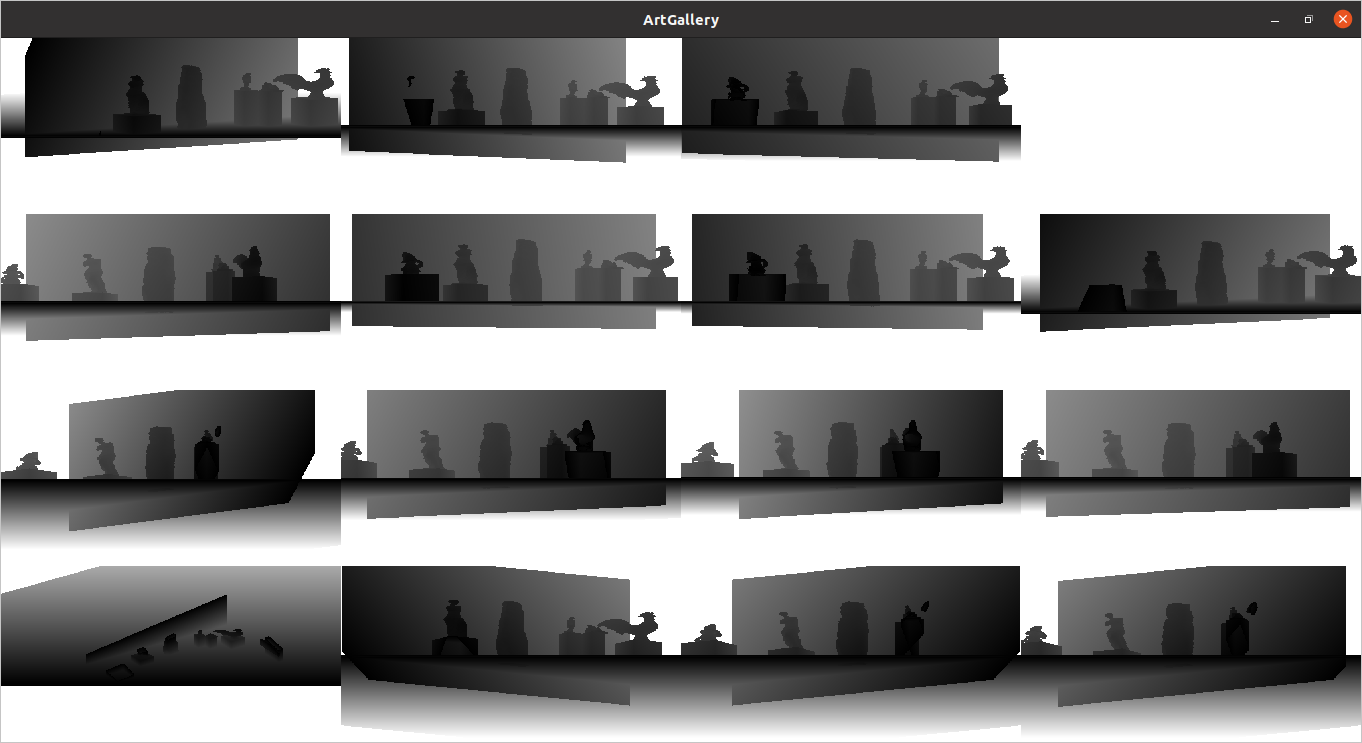
\includegraphics[scale=0.5]{images/mapasombra.png}
\caption{Mapa de sombras generado}
\end{figure}


\section{Estructura del código}


 \subsection{Object}
Almacena la informaciòn del objeto a renderizar. Esto incluye coordenadas de los vertices, definición de las caras del poligono (por medio de indices a los vertices), normales de las caras, normales de los vértices, coordenadas UV e informaciòn sobre el material (coeficientes ka,kd,ke)

En el constructor de la clase de define el material a utilizar. En los materiales también se puede cargar una textura, correspondiente a ese material.

Esta clase también tiene mètodos para realizar rotaciòn de euler en $x$, $y$ y $z$, y para calcular las normales de las caras y de los vértices. La información de las normales también se puede almancenar desde un archivo OBJ.

Por otro lado, por medio del método render se dibuja el objeto con glDrawElements. LA misma función se encarga de manejar el envio de datos en el vertex buffer.


\subsection{lights}
La clase \textit{lights} almacena la informaciòn de las luces de la escena. Se define:
\begin{itemize}
\item Tipo (de sol o spotlight)
\item Posición
\item Dirección
\item Color
\item angulo de corte (para spotlights)
\item intensidad
\end{itemize}

\subsection{mainWindow}
La clase de la ventana principal maneja todas las funciones para renderizar la escena.
En \textit{mainwindow.cpp} se crea el contextro de opengl, se importan los objetos, se inicializan los parámetros de las luces y la posición de la cámara.
 Después en \textit{InitializeGL} se compilan los shaders con la función compileShaders. Posteriormente se crea el framebuffer y se liga su textura para dibujar profundidad
 FInalmente en paintGL se dibuja la escena sobre el framebuffer principal. Primero el ambiente con \textit{renderEnviroment} y después la escena con \textit{renderScene}
 
 En general el proceso para renderizar un objeto es el siguiente. Si se utiliza textura se llama a setTextures, dando como argumento u string con el 'path' de la textura. Después se envían las variables necesaria al shader. Pra Phong se utliza setShaderValues. Finalmente se llama a renderizar al objeto con el método render de la clase Object.
 
\textbf{$$maindown\_scene.cpp$$}
Contiene la función setScene() que importa losmodelos obj, inicializa su posición y transformaciones necesarias, modificando su matriz de modelo. 

\textbf{$$mainwindow\_setShader.cpp$$}
Contiene la función compileShaders y funciones específicas de cada shader para recibir las variables necesarias por el programa, por medio de glUniform.

\textbf{$$mainwindow\_shadowMap$$}
Contiene la función genDepthMap()para generar el mapa de profundidad que permita realizar shadowmapping. D igual manera, la función renderShadowMapDebug() que sirve para debugiar el mencionado mapa de sombras.
{

\section{Ejecutar el programa}
En la carpeta de build se puede ejecutar el programa con el archivo ArtGallery-Run. Desde la consola de comandos de linux:

\begin{lstlisting}[language=bash,title={bash}]
./ArtGallery-Run
\end{lstlisting}


En la carpeta principal está el código fuente. Para generar el ejecutable primero se genera el Makefile con

\begin{lstlisting}[language=bash,title={bash}]
 qmake ArtGallery.pro
\end{lstlisting}

Después se construye el proyecto con \textit{make}

\section{Instrucciones de uso}
Se presenta la interfaz del programa.


Para navegar por el escenario se utilizan 2 juegos de teclas.
Primero para cambiar la posición:
\begin{itemize}
\item "W". Moverse hacia enfrente
\item "A". Moverse la izquierda
\item "S". Moverse hacia atrás
\item "D". Moverse hacia la derecha
\end{itemize}

Para cambiar la dirección (hasta 90º):

\begin{itemize}
\item "I". Girar hacia arriba
\item "J". Girar hacia la izquierda
\item "K". Girar hacia abajo
\item "L". Girar hacia la derecha
\end{itemize}

Para apagar las luces que iluminan los objetos se utilizan las teclas de número del 1 al 8.
Cada tecla apaga la luz correspondiente a ese número de objeto. Debido a la manera en que están indexadas las luces apagar más de una a la vez provoca comportamiento erratico.

Para desactivar shaders
\begin{itemize}
\item \textit{B} desactiva reflect shader
\item \textit{N} desactiva toon shader
\item \textit{M} desactiva movement shader (textura animada)
\end{itemize}

Volverlo a presionar hace que se activen de nuevo. 

\section{Resultados}

El programa se corriò en un computadora con procesador AMD FX-8370, con tarjeta gráfica Nvidia GTX 970 y 12 gb de memoria ram. 

\begin{figure}[H]
\centering
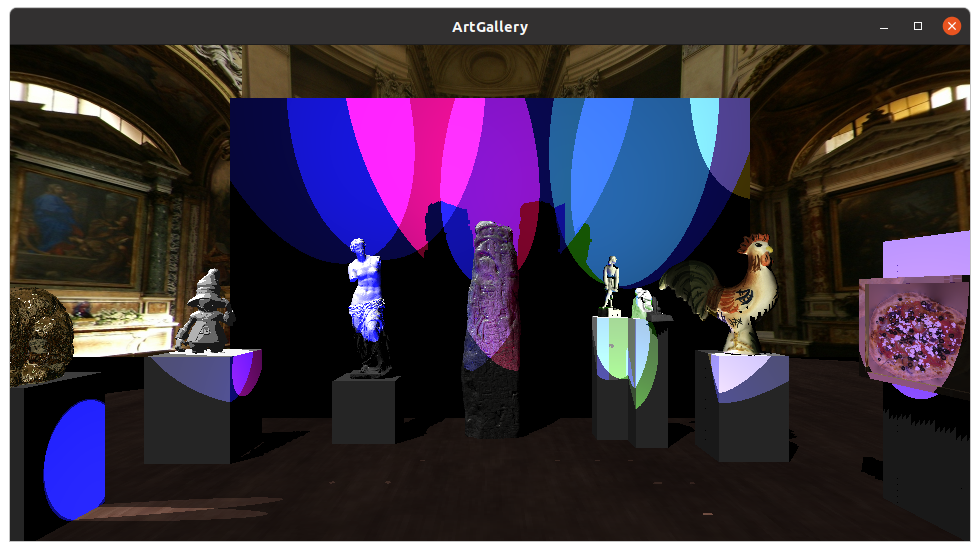
\includegraphics[scale=0.5]{images/inicio.png}
\caption{Escena que se muestra la iniciar el programa}
\end{figure}

\begin{figure}[H]
\centering
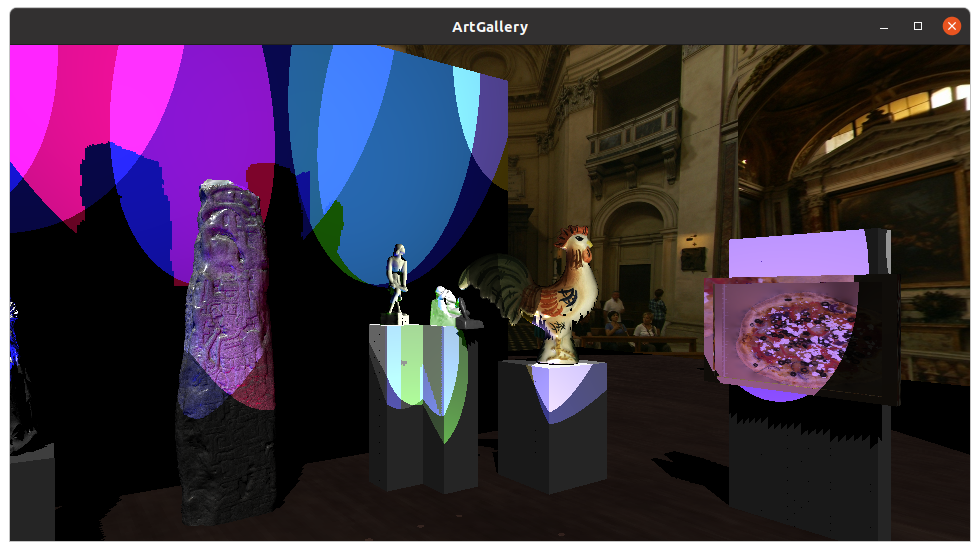
\includegraphics[scale=0.5]{images/der.png}
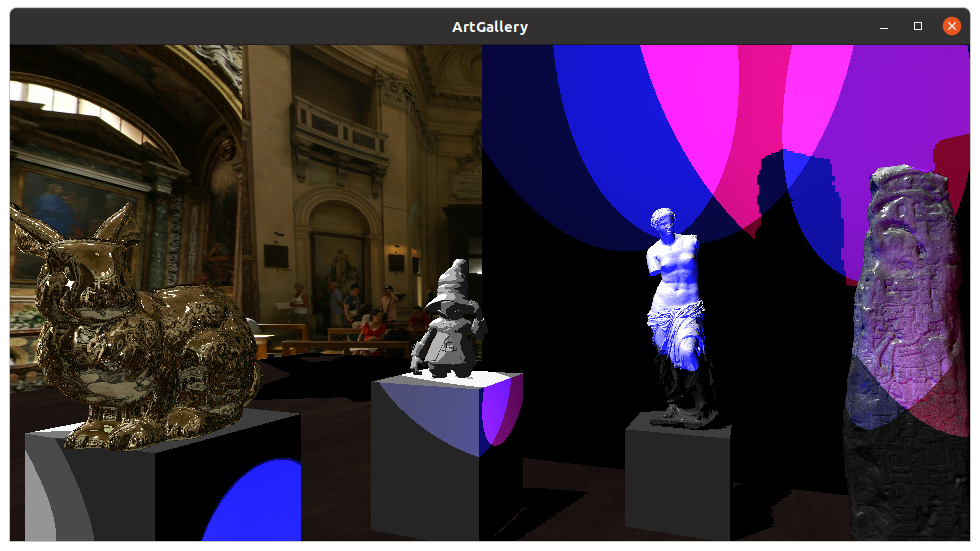
\includegraphics[scale=0.5]{images/izq.png}
\caption{Galería de arte}
\end{figure}

\begin{figure}[H]
\centering
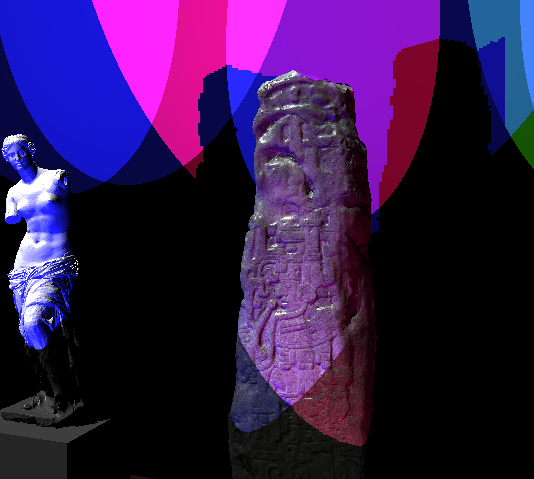
\includegraphics[scale=0.5]{images/luzon.png}
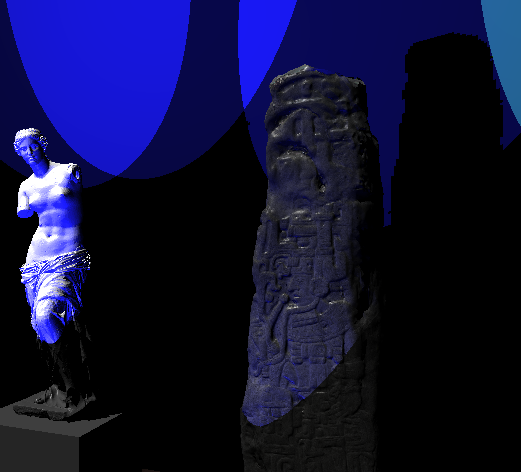
\includegraphics[scale=0.5]{images/luzoff.png}
\caption{Desactivación de luces}
\end{figure}

\begin{figure}[H]
\centering
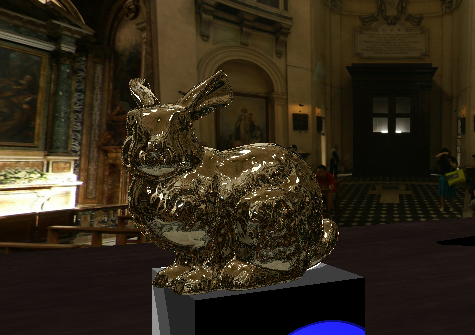
\includegraphics[scale=0.5]{images/reflec.png}
\caption{Mapeo ambiental reflectivo}
\end{figure}

\begin{figure}[H]
\centering
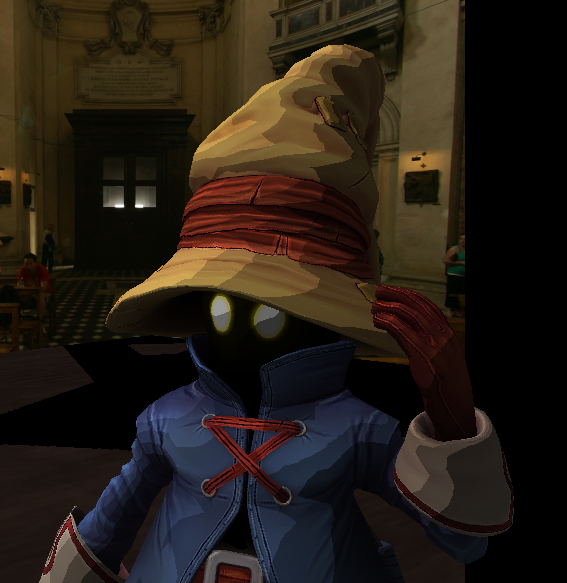
\includegraphics[scale=0.4]{images/toontex.png}
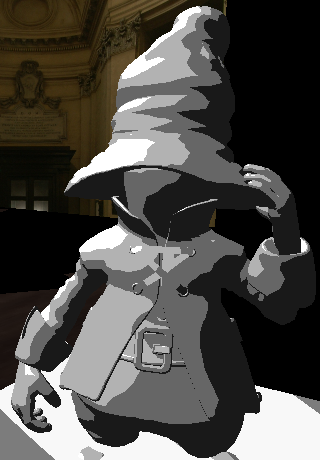
\includegraphics[scale=0.5]{images/toon.png}
\caption{Toon shader con y sin textura}
\end{figure}

%\begin{thebibliography}{99}



\end{document}